\documentclass[10pt]{exam}
\usepackage[icp]{template-for-exam}
\usepackage{tikz}
\usepackage[top=0.5in, bottom=0.5in, left=1in, right=1in]{geometry}


\begin{document}
\pagestyle{empty}

\newcommand{\topmatter} {
  {\noindent \Large \bf Unit P2 Test - Measurement}

  \vspace{3em}

  \noindent {\bf Please do not open this test until told to do so!}

  \begin{itemize}
    \item Put your name on both the front \emph{and} the back of this page.
    \item Bubble in the number that is on your class notebook where it says “Student ID”
    \item When instructed, tear off this first page.
    \item Write your answers to the free-response questions directly on the packet.
    \item Bubble in your answers to the multiple-choice questions here.
    \item You may write anywhere on the packet.
    
  \end{itemize}

  \noindent {\bf When you are finished,}

  \begin{enumerate}
    \item Turn your test face down in front of you (Don't get up to turn it in).
    \item Sit silently until everyone is done.
    
  \end{enumerate}
}
\newcommand{\bottommatter}{
  \begin{flushright}
    
\begin{tikzpicture}
      \draw (-0.3,0) -- (0.3,0) -- (0,0.530) -- cycle;
      \node at (0,0.2) {\bf !};
    \end{tikzpicture}
    \bf Don't forget to answer the problems on the back!! $\bf \Longrightarrow$
  \end{flushright}
}

\newcommand{\scantron}[2]{
  \begin{flushright}
    \begin{tikzpicture}
      \node[anchor=south west] at (0,0) {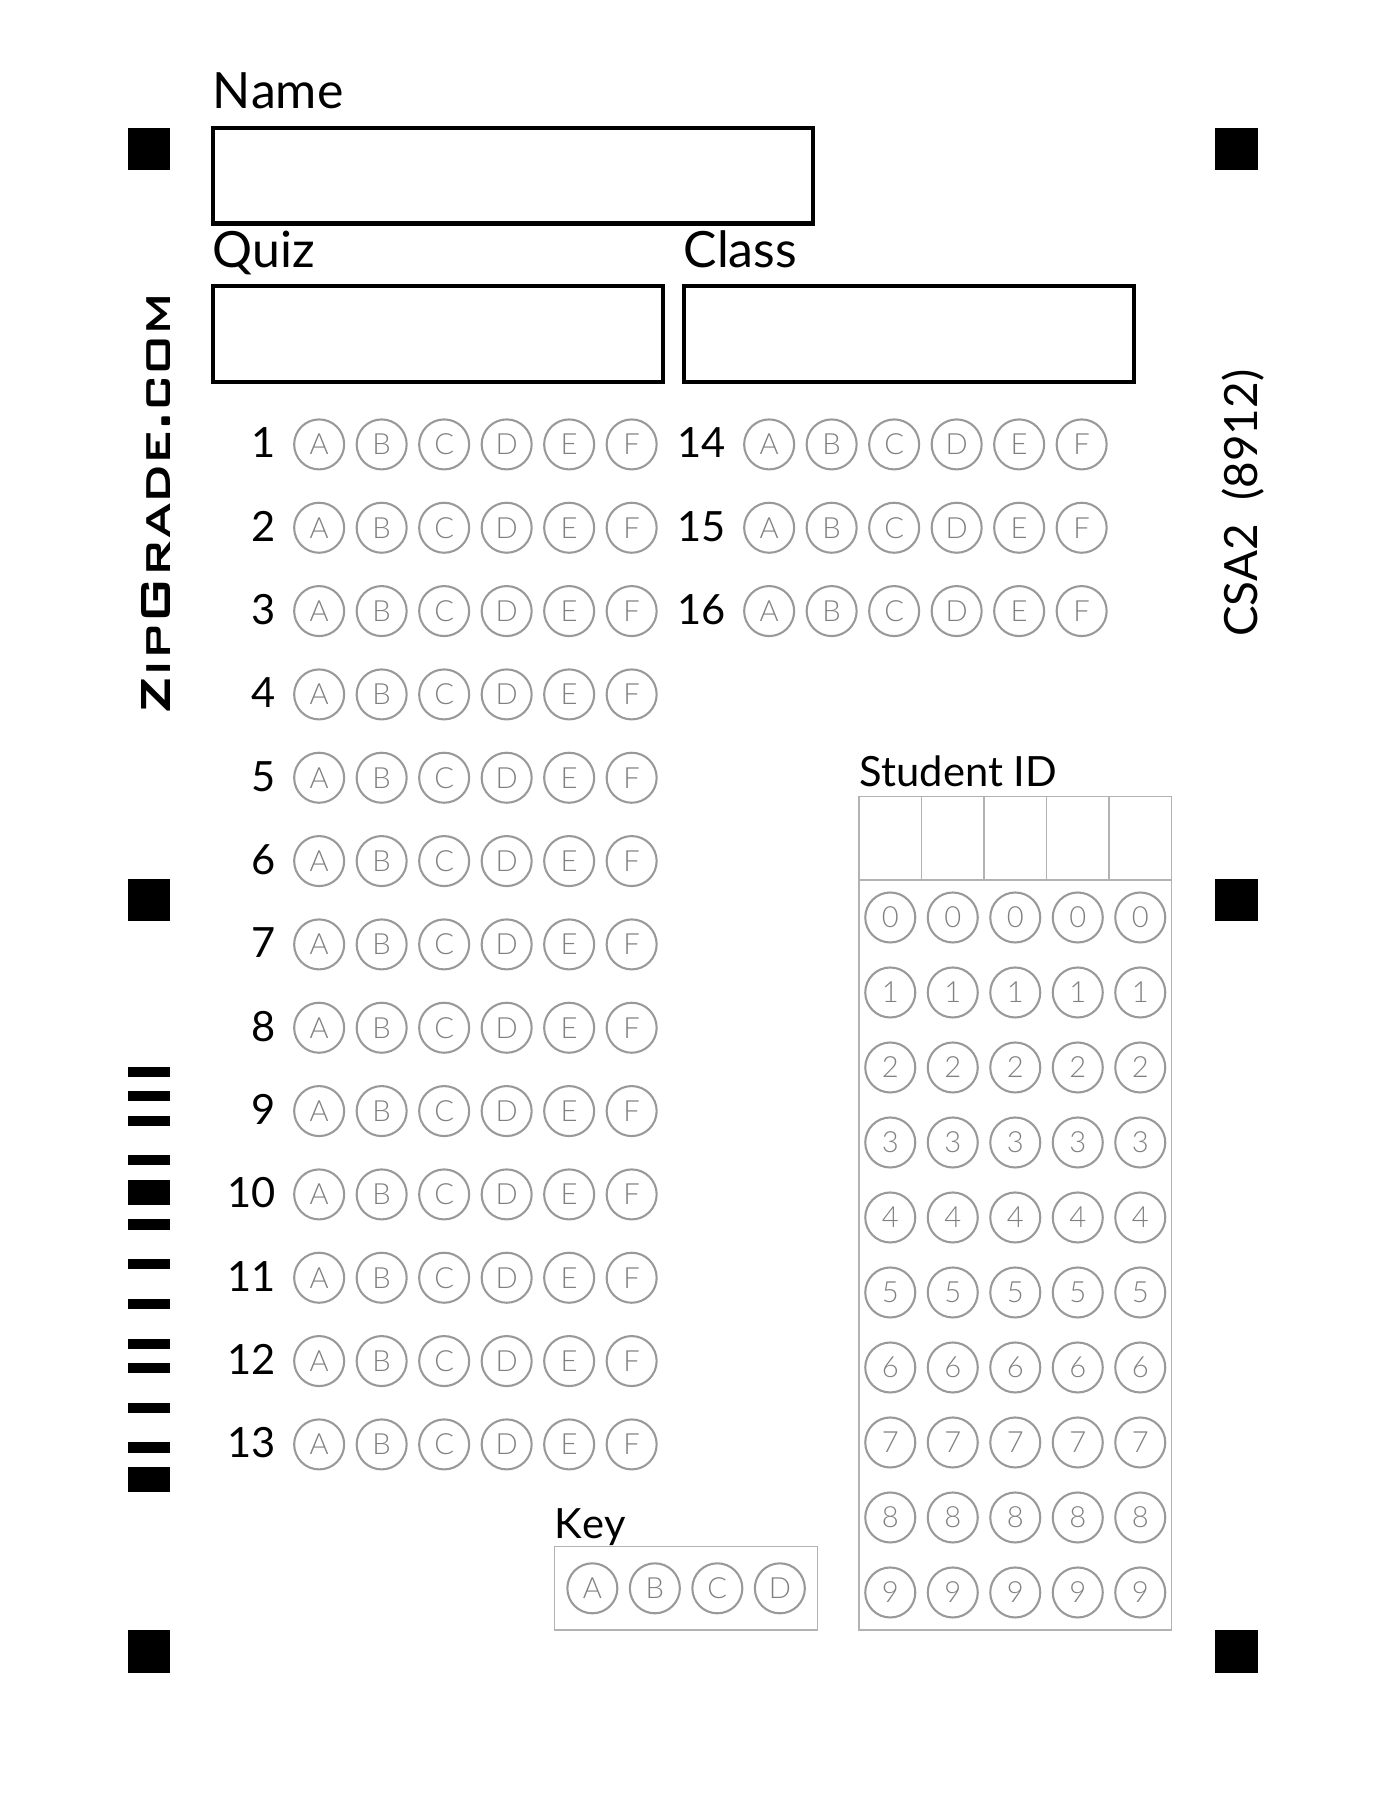
\includegraphics[width=4in]{scantron.png}};
      \fill (#1,#2) circle (0.2);
      \node[anchor=west] at (1.6,10.8) {\small P2 (Measurement) Test};
    \end{tikzpicture}
  \end{flushright}
}


\scantron{5.25}{1.7}
\bottommatter
\topmatter
\pagebreak
\scantron{5.75}{1.7}
\bottommatter
\topmatter
\pagebreak
\scantron{6.24}{1.7}
\bottommatter
\topmatter
\pagebreak
\scantron{6.73}{1.7}
\bottommatter
\topmatter


\end{document}